\documentclass[tikz,border=3pt]{standalone}
\usepackage[utf8]{inputenc}
\usepackage[T1]{fontenc}
\usepackage{lmodern}
\renewcommand{\familydefault}{\sfdefault}
\usepackage{sansmath}\sansmath
\usepackage{chemfig}
\usepackage{pgfplots}\pgfplotsset{compat=1.18,/pgf/number format/use comma,/pgf/number format/1000 sep={.}}
\usetikzlibrary{arrows.meta,calc,positioning,decorations.pathmorphing,patterns}
% paleta del sitio
\definecolor{nar}{HTML}{E8680C}\definecolor{narc}{HTML}{FFB35C}\definecolor{hielo}{HTML}{FFF3E8}
\definecolor{tinta}{HTML}{1D1D1F}\definecolor{gris}{HTML}{6E6E73}\definecolor{lila}{HTML}{7C5CF0}
\definecolor{azul}{HTML}{2F6FD6}\definecolor{menta}{HTML}{17A673}\definecolor{coral}{HTML}{E8342A}
\tikzset{cel/.style={draw=gris,fill=hielo,line width=0.9pt},nuc/.style={draw=gris!70,line width=0.6pt},
fib/.style={gris!55,line width=0.35pt},eti/.style={font=\footnotesize,text=tinta,align=center},
num/.style={circle,draw=nar,fill=white,text=nar,font=\small\bfseries,inner sep=1.2pt,minimum size=13pt},
fl/.style={-{Stealth[length=2.6mm]},gris,line width=0.9pt}}
\begin{document}
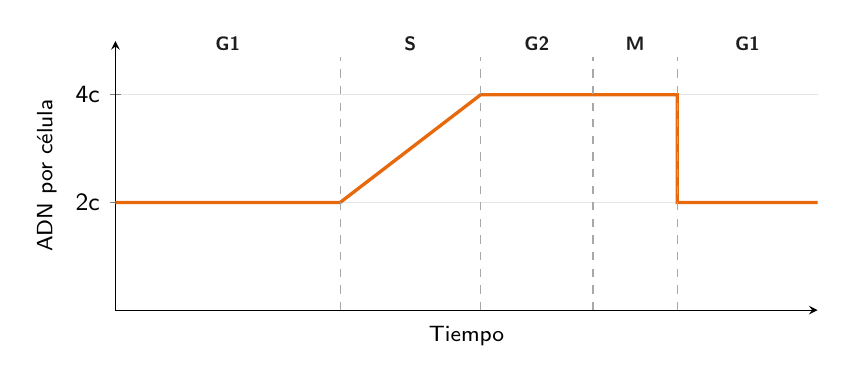
\begin{tikzpicture}[font=\small]
\begin{axis}[width=10.5cm,height=5cm,axis lines=left,xmin=0,xmax=12.5,ymin=0,ymax=5,xtick=\empty,ytick={2,4},yticklabels={2c,4c},
xlabel={Tiempo},ylabel={ADN por célula},ylabel style={font=\footnotesize},xlabel style={font=\footnotesize},clip=false,ymajorgrids,grid style={gray!20}]
\addplot[nar,very thick] coordinates {(0,2) (4,2) (6.5,4) (8.5,4) (10,4) (10,2) (12.5,2)};
\draw[gris!60,dashed] (axis cs:4,0)--(axis cs:4,4.7);
\draw[gris!60,dashed] (axis cs:6.5,0)--(axis cs:6.5,4.7);
\draw[gris!60,dashed] (axis cs:8.5,0)--(axis cs:8.5,4.7);
\draw[gris!60,dashed] (axis cs:10,0)--(axis cs:10,4.7);
\node[font=\scriptsize\bfseries,text=tinta,align=center] at (axis cs:2,4.95) {G1};
\node[font=\scriptsize\bfseries,text=tinta,align=center] at (axis cs:5.25,4.95) {S};
\node[font=\scriptsize\bfseries,text=tinta,align=center] at (axis cs:7.5,4.95) {G2};
\node[font=\scriptsize\bfseries,text=tinta,align=center] at (axis cs:9.25,4.95) {M};
\node[font=\scriptsize\bfseries,text=tinta,align=center] at (axis cs:11.25,4.95) {G1};
\end{axis}
\end{tikzpicture}
\end{document}
